%!TEX TS-program = /opt/local/bin/pdflatex
% TEMPLATE for Usenix papers, specifically to meet requirements of
%  USENIX '05
% originally a template for producing IEEE-format articles using LaTeX.
%   written by Matthew Ward, CS Department, Worcester Polytechnic Institute.
% adapted by David Beazley for his excellent SWIG paper in Proceedings,
%   Tcl 96
% turned into a smartass generic template by De Clarke, with thanks to
%   both the above pioneers
% use at your own risk.  Complaints to /dev/null.
% make it two column with no page numbering, default is 10 point

% Munged by Fred Douglis <douglis@research.att.com> 10/97 to separate
% the .sty file from the LaTeX source template, so that people can
% more easily include the .sty file into an existing document.  Also
% changed to more closely follow the style guidelines as represented
% by the Word sample file. 
% This version uses the latex2e styles, not the very ancient 2.09 stuff.
\documentclass[letterpaper,twocolumn,10pt]{article}
\usepackage{float,usenix,epsfig,endnotes,graphicx}

\renewcommand{\topfraction}{0.9}	% max fraction of floats at top
\renewcommand{\bottomfraction}{0.8}	% max fraction of floats at bottom

\begin{document}

%don't want date printed
\date{}

%make title bold and 14 pt font (Latex default is non-bold, 16 pt)
\title{\Large \bf Intellidrive: Improving Disk Drive Read Access with Machine \\ Learning Algorithms}

\author{
{\rm Peter Gebhard}\\
\and
{\rm Philip Joseph}\\
University of Illinois at Urbana-Champaign \\
Department of Computer Science
\and
{\rm Vance Thornton}\\
} % end author

\maketitle

% Use the following at camera-ready time to suppress page numbers.
% Comment it out when you first submit the paper for review.
\thispagestyle{empty}

\begin{abstract}
A more efficient approach to performing disk drive read accesses is explored.  In this approach, a machine learning algorithm is used to optimize the positioning of data on a disk and the effectiveness of precaching based on information about the patterns of access to data on the disk.  The goals of these optimizations are to reduce the number of random data read operations performed and to better utilize disk idle time.  The Intellidrive architecture consists of a disk driver to log read and write requests coming from the file system and an optimizer program which uses the generated access logs as input to its algorithm.  The optimizer program performs block reorganization by updating the virtual to physical block map used by the disk driver and forms groups of data that should be precached together.  Results indicated that there was a sufficient amount of random reads to exploit; however, the current Intellidrive implementation using a genetic algorithm saw no appreciable improvement.
\end{abstract}

\section{Introduction}
In the unwavering demand for ever faster computing, we have grown accustomed to a relatively stagnant rate of improvement in hard disk drive access times ~\cite{CachingStrategies}.  Meanwhile, advances in CPU, GPU, and RAM technologies continue to push the limits of performance.  Because a hard drive is a mechanical device with moving parts data access time is highly dependent on the location of the data on the disk.  Data that is read from sequential block locations can be read many times faster than data that is read from random block locations.  It is from these observations that we are focusing on a method to alleviate the disk drive from its mechanical limitations and improve it's perceived performance through adaptive block organization and data precaching which attempts to minimize the number of random data read operations performed and to better utilize disk idle time.

In current approaches much of the responsibility for data access performance is placed on the application developer.  Decisions regarding the use of files and the organization of data within files can have a significant impact on data access performance.  Choosing an appropriate data organization can be a difficult task that is even more difficult when it is not known in advance what the common access patterns will be.  Current approaches attempt to ease this burden by providing caching based on simple assumptions such as that data that was accessed recently is more likely to be accessed again soon and that data that is near data that is being read in a file is likely to be read soon.  Existing file system implementations attempt to reorganize data so that files are stored sequentially on the disk.  Whether or not these assumptions about disk access patterns and appropriate block organization are correct is highly application dependent and may change over time.

The typical approach to solving data latency issues is to build a caching store as a new layer between the requester and the requestee.  To improve disk drive access performance, modern hard disk drives now commonly include a read/write disk buffer that allows the disk drive to cache sectors ahead of (and possibly behind) a requested sector read ~\cite{MultiplePrefetch}.  This same disk buffer can also be used to queue incoming write requests so the system's OS can continue other processing.  So while most system disks already contain a disk buffer, we feel that disk read performance can be improved by moving beyond a simplistic read-ahead approach and instead applying a machine learning algorithm.  Our approach will not focus on any significant changes to how write requests are queued and scheduled.

Our approach has the potential to be better than current approaches because the access pattern prediction utilizes more sophisticated models that are based on access history and adapt over time.  By providing adaptive block reorganization we will also hopefully reduce or eliminate the need for application developers to consider the performance implications of data organization as data organization will adapt over time based on usage.

\begin{figure*}[ht]
  \center{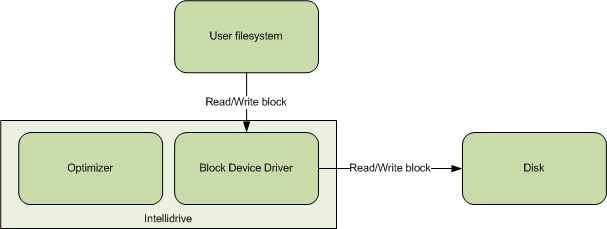
\includegraphics[width=\textwidth]
  {system-architecture.png}}
  \caption{Intellidrive System Architecture}
\end{figure*}

The anticipated eventual result of this project is that disk read performance will be improved for tasks that require repeated random I/O for sets of related data.  Improving write performance is not a goal of this project, however a potential benefit of intelligent block reorganization is that random writes can be replaced with sequential writes which are later reorganized based on access patterns.

\section{Design}
\subsection{System Architecture}
The Intellidrive system is composed two main components, a block device driver and an optimization utility.  The user file system makes use of the Intellidrive block device driver to store information.  The Intellidrive block device driver processes the requests from the file system and uses the physical disk for block storage.  In addition to servicing block read/write requests the driver performs device access logging and block precaching.  The optimization utility uses machine learning to attempt to improve the block organization and precache groups.  An overview of the Intellidrive system architecture is shown in Figure 1.

\subsection{Logical to Physical Block Mapping}
In order to support intelligent block reorganization Intellidrive maps logical block numbers to physical block numbers.  This is implemented using an array where the value stored at element N is the physical block number of logical block number N.  If 4KB blocks are used this map requires 1 megabyte of memory for every gigabyte of drive storage capacity. 

When a read request with logical block numbers comes in, our program uses the mapping to create an array of the corresponding physical block numbers.  That array is then sorted, and the reads of the physical blocks are performed (combining reads of consecutive blocks into one read call).

This mapping array is created from a file that is stored on a separate drive.  Originally the file is an in order mapping of logical to physical blocks.  When run, the algorithm will move the physical blocks on the disk and update the mapping file to match the new ordering.

\subsection{Precache Boundaries}
Intellidrive makes use of precache groups to represent groups of blocks that should be precached together.  During drive idle time blocks sequentially following recently read blocks are precached into memory until a precache boundary is reached.  The precache boundaries are represented using a bit vector where the bit stored at position M in the vector has a value of 1 if precaching should stop after block number M has been precached.  Represented as a bit vector the precache boundaries require 32KB of memory for every Gigabyte of drive storage capacity.

\subsection{Device Access Logging}
Logging data will be the main input to our algorithm.  Currently we log every read access to the drive.  We are not logging any writes.  The format of the log is simple.  Each log consists of two 32-bit entries.  The first entry is the timestamp.  The second entry is the block number that is read.

See Figure 2 for an example structure that could represent the data that is going to be logged.

\begin{figure}[htb]
  \center{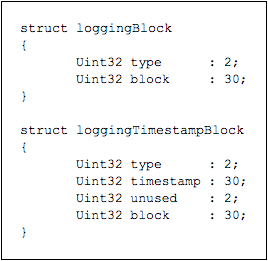
\includegraphics[width=3in]
  {code.png}}
  \caption{Example Logging Data Structures}
\end{figure}

\subsection{Drive Optimization}

A genetic algorithm ~\cite{GeneticAlgorithm, GAlib} is used to optimize the drive by intelligently reorganizing blocks and redefining precache groups on a periodic basis.  The process begins with an initial population of randomly generated organisms.  Each organism is represented by a logical to physical block mapping and the boundaries of the precache groups.  The fitness of each organism is calculated based on the efficiency with which the accesses in the logs would have been able to be performed given the organism’s block mapping and precache groups.  Performance on older logs contributes less to fitness than performance on newer logs and the similarity of an organism to the current block organization and the logical block organization are also included in the fitness measure.  The most fit organisms are mated with a small probability of mutation to produce the next generation of organisms.  In the mating process the traits being expressed are precache groups.  Each offspring will have some combination of the precache groups of its parents.  In order to ensure that an offspring maps each logical block to one and only one physical block when a precache group is added from one parent all of the already used physical blocks in that group are removed.  Removing these blocks will result in precache groups that become smaller over time.  In order to counteract this if the size of a precache group falls below a specified threshold that group is merged with the group that precedes it.  If the size of a precache group exceeds a specified threshold that group is split into smaller groups.  An example of the combination of two parents to form an offspring is shown in Figure 3.

\begin{figure}[htb]
  \center{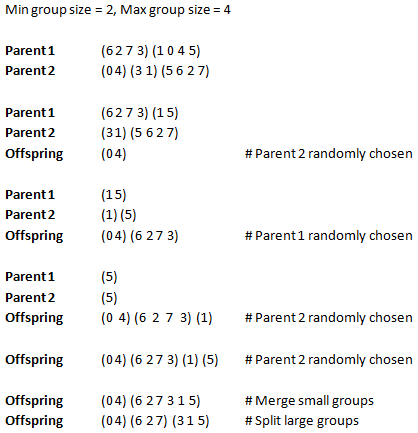
\includegraphics[width=3in]
  {ga-combination.png}}
  \caption{Genetic Algorithm Combination}
\end{figure}

The fitness of each generation is calculated and the organisms are mated to produce the next generation until a specified amount of time has elapsed or the fitness of the most fit individual does not improve for a specified number of generations.  The physical blocks are then reorganized to reflect the ordering specified by the mapping of the most fit organism and the precache boundaries are replaced with those of the most fit organism.

\section{Current Status}

We have a functional implementation of the Intellidrive device driver which works with reorganized blocks stored on the disk, logs access information to files, and performs precaching.  We have also implemented a genetic algorithm for drive optimization, but our current implementation is too slow to be practicably usable.

\section{Implementation}
\subsection{Initial Implementation}
We ran into quite a bit of trouble when trying to implement our design.  We initially started with a Linux Block Device Driver and an Algorithm written in Java.  The algorithm written in Java didn't impose too many problems, but we ran into significant delays in trying to develop the driver.  With limited documentation, developing in the kernel proved to be difficult.  We attempted a user space daemon that would minimize kernel code, but we had problems getting network traffic to work in order to implement the user space daemon.  We then decided to move our development of the driver to a Java iSCSI target.  Once again we had troubles getting the user space daemon to work with this code.

\subsection{Final Implementation}
Due to the good documentation that we could find for Windows, we moved our coding efforts to a Windows driver (all based in the kernel).  We used C for the driver.  We also decided to move our algorithm to C++ to make use of an existing genetic algorithm framework.  We also coded a drive loader in C++ to mount the drive.

\subsection{Usage}
In order to use our code, it is necessary to do some minimal installation, including copying a file to the system directory and installing some registry keys.

After restarting the system, you can use our drive loader to mount the drive as a normal windows drive (ie, the G drive).

From there, you can use this new drive as normal (such as copying/moving/deleting/ and running files on it).  When the drive is idle for a while or upon restart, the drive is unmounted and the algorithm is run on the drive.  The algorithm will rearrange the blocks and create a mapping file that will get read in when the drive is mounted.  This mapping will allow programs to continue to use the drive as if the blocks haven't moved.

\section{Evaluation}
\subsection{Experiments and Results}
In order to have a better understanding of the potential performance gains from intelligent block reordering, we first used a tool called Iometer to measure read/write performance of a typical hard drive. As expected we found significant disparity between sequential and random read performance.  From the following table you can see that sequential reads were almost 75 times faster than random reads when a 4k request size was used.
 
\begin{center}
  \begin{tabular}{ | c | c | }
    \hline
    \textbf{Read Types} & \textbf{Disk Drive Performance} \\ \hline
    Sequential & $\sim$11.0MB/s \\ 
    Random & $\sim$0.15MB/s \\
    \hline
  \end{tabular}
\end{center}

As the implementation of our algorithm focuses on improving read access times, we also focused our attention on tasks that involved a large amount of disk reads.  We used the logs from our Intellidrive device driver to profile the access patterns in some common usage scenarios. 

In doing our measurements, we minimized the chance that the OS cache introduced too many variables in our measurements, by running our tests on fresh reboots to make sure we are working with a clean cache in order to accurately measure our performance.  Figure 4 shows some of the results that we measured.

\begin{figure*}[htb]
  \center{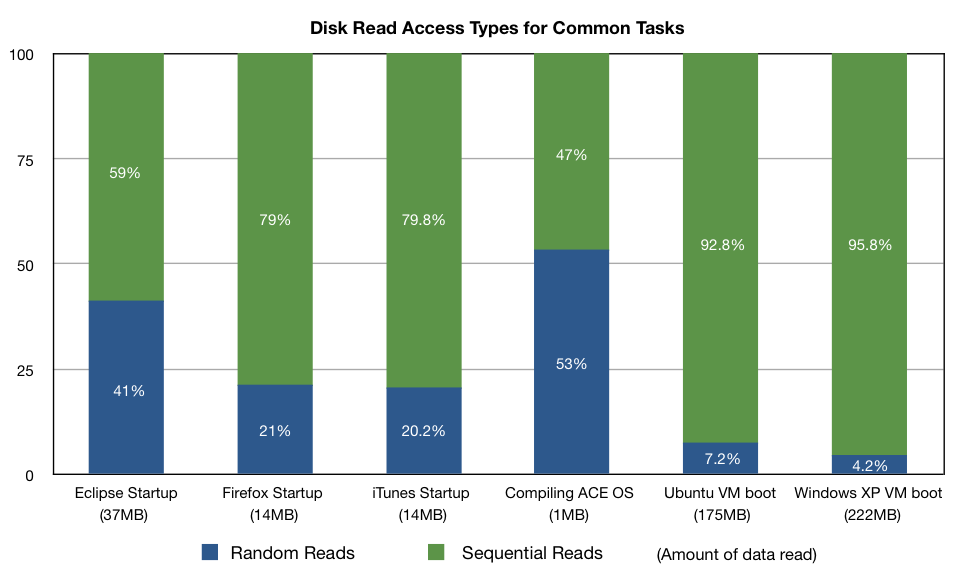
\includegraphics[width=\textwidth]
  {ScenarioChart.png}}
  \caption{Read Types for Common Tasks}
\end{figure*}
 
From the figure, it can be seen that applications can often perform a appreciable number of random reads during startup.  This indicates that startup performance would likely be improved by more efficient block organization and precaching if disk I/O is a bottleneck to startup.  Our logs of operating system boot in a virtual machine suggest that the read access patterns are already quite efficient with some, but not much room for improvement.

We have not been able to determine the actual performance impact of using the Intellidrive system.  This is because we have found that with our current genetic algorithm formulation, the fitness of the population does not improve quickly enough to be practically useful.  We have attempted to improve the algorithm by changing various parameters used as well as the fitness and mating functions.  An example of one of these changes was to make the fitness function more discriminative by incorporating the distance between random reads.  Our current hypothesis is that the size of the organism representation and the amount of data involved determining fitness is too great to make the use of a genetic algorithm feasible.

\section{Related Work}
While disk caching is not a particularly new idea, it is still an important area of study in computing systems as disk access times continue to be outpaced by other technological advances ~\cite{MultiplePrefetch}.  As disk access times have stagnated, though, disk capacity has grown dramatically.  The dynamics of this trade off has led systems to exploit caching where possible.  Some of the ideas that are being explored in our own research have also been studied in the past by other related work, so that is why the primary focus of our effort has been on the application of machine learning algorithms in this domain.  Some related work included elements of machine learning in their basic caching and rearrangement algorithms, but these were not the main focus of their study.  The following work helped us direct and adapt our own study as we learned the techniques that had been used in the past.  Overall, it was surprising that much of this prior work was performed at least a decade ago, but despite the notion that disk caching was already a solved problem, we felt that there might still be room for improvement through use of more advanced algorithms.

In work by Grimsrud, Archibald, and Nelson ~\cite{MultiplePrefetch}, we studied how they had developed new approaches of using prefetching schemes to improve disk access performance.  Their scheme was designed to be more sophisticated than simple precaching of disk blocks ahead of those currently being read.  Instead, they developed prefetching that could adapt its efforts based on what it had seen in prior disk accesses.  Its role in detecting useful disk access patterns would in turn result in more efficient prefetching decisions for future disk accesses.

The main avenues for disk access optimization in our design are through effective prefetching and block rearrangement.  Therefore, it was very important for us to understand how existing prefetching strategies work, as well as how to avoid any of the pitfalls that previous researchers had faced.  A key point made by Grimsrud, et al., is that one must be diligent about ensuring reliable accuracy when prefetching, for a poorly design prefetching scheme can decrease disk performance due to pollution of the cache and unexpected congestion.  Another key concept from this paper comes from their use of an adaptive table which stores the most likely successive disk accesses after a particular block has been accessed.  This concept can be much more effective than simply prefetching blocks sequentially beyond the particular block.

Our approach to implementing and testing our algorithmic improvements to disk drive read accesses was to develop a disk block device driver for Linux.  By using a disk driver, the physical drive and partitions were abstracted and we could control a layer below the file system.  In controlling this layer, we decided that using a logical to physical block mapping would give us precise, low-level control over which blocks would be accessed whenever the file system presented a request.  At the same time, this mapping would give us the ability to perform block rearrangement virtually without ever having to physically move disk blocks if so desired ~\cite{Loge}.  We researched work on the Logical Disk (LD) by de Jonge, Kaashoek, and Hsieh ~\cite{LogicalDisk} to help us understand what concepts were found to be important in developing a system with this type of indirection mapping.  The Logical Disk was shown to deliver a useful abstraction layer without a detrimental effect on efficiency.  This added layer does not come completely free, as there is added storage overhead required in order to maintain the logical to physical block mapping.

Finally, we studied the work of Akyurek and Salem on Adaptive Block Rearrangement ~\cite{AdaptiveBlock}.  Block rearrangement will be one of the most important functions of our technique, as it is the efficient placement of blocks that will in turn allow for reduced disk access times when disk requests are made and precaching is in use.  In Akyurek and Salem's work, their adaptive algorithm requires no prior knowledge of the type of information it will encounter in order to perform effectively, and with our use of a genetic algorithm, our method will not require prior knowledge to perform either.  Our technique, however, does differ from Akyurek and Salem's in how it adapts to the incoming information stream.  While their algorithm merely uses frequencies to estimate which block will most likely follow a given block, we use a more sophisticated, genetic algorithm that learns as it continues to process new disk requests.  This difference marks our primary goal of determining if advanced machine learning algorithms can improve disk drive read access performance.

\section{Future Research}
There are several areas in which the research presented in this paper could be improved.  One area would be continued investigation to determine if a genetic algorithm can be practically applied to solve this problem.  This would involve work to determine the impact of the size of the organism representation and the amount of log data on the time required to find an efficient block organization and precache groupings.  Another area would be in applying more machine learning algorithms to this problem to evaluate potential tradeoffs between the time to find a solution and the efficiency of that solution.

In this paper we did not attempt to improve write performance, but the flexibility of the block mapping used in this approach makes it possible to reduce or eliminate random writes by writing data sequentially and updating the block mapping appropriately.  An interesting aspect of the research involved in doing this would be in determining a method for ensuring that there are a sufficient number of contiguous blocks available for this purpose.

Finally an important aspect of this work that will need to be investigated is the evaluation of the performance impact of using this approach.  It is not necessarily appropriate to use conventional benchmarks to test this approach because it relies on access patterns which may be overly random or too predictable in a typical benchmark.  The approach is also adaptive so a single execution of a benchmark may not give a completely accurate indication of the results.  Our initial inclination is that benchmarks based on logs captured from real world situations will be most useful in performance evaluation.

\section{Conclusions}
We have described our Intellidrive system which was designed to improve disk drive read access times using machine learning algorithms. Although we were not able to use a genetic algorithm to obtain an optimized block ordering or precache groups, we are still convinced that this area has other possibilities of success.  

As hard drive speeds have consistently been a bottleneck in computer speeds, this area of research could prove to be a very important one.  While existing research has touched on some of the techniques that we employed in Intellidrive, our system uses more advanced techniques that should be able to provide improved results.

We believe that with a little more time or manpower, variations on our implementation of the genetic-algorithm-based Intellidrive or the use of different machine learning algorithms in the system could prove to be more successful.

{\footnotesize \bibliographystyle{acm}
\bibliography{./final}}

\end{document}







